\clearpage
\phantomsection

\setcounter{chapter}{1}
\chapter[{NHẬN DẠNG HỆ THỐNG SỬ DỤNG THUẬT TOÁN BÁN MÙ MRE}]{Nhận dạng hệ thống sử dụng thuật toán bán mù MRE}
\label{sec:MRE}

Trong chương này, trước hết, tác giả sẽ trình bày các tìm hiểu sơ lược về một thuật toán ước lượng kênh truyền mù truyền thống là bộ cân bằng kênh tham chiếu (MRE - Mutually referenced equalizers). Giải thuật B-MRE sẽ được phát triển để hoạt động với các hệ thống MIMO. Sau đó, phương pháp SB-MRE được đề xuất bằng cách sử dụng thêm một số lượng nhỏ pilot cùng với thông tin từ B-MRE. Sau đó, các hai phương pháp nhằm giảm thiểu chi phí của thuật toán SB-MRE được đề xuất, bao gồm giảm độ phức tạp của B-MRE và giảm thiểu độ dài chuỗi pilot. Cuối cùng, các mô phỏng được thực hiện để kiểm chứng thuật toán đề xuất và đưa ra kết luận.

\section{Sơ lược về thuật toán B-MRE}

Trong luận văn này, thuật toán bộ cân bằng kênh tham chiếu (MRE - Mutually referenced equalizers)~\cite{original} được lựa chọn để phát triển theo hướng tiếp cận SB. Giải thuật gốc đã được đề xuất từ năm 1997 bởi Gesbert D. và các đồng tác giả. Lý do lựa chọn MRE là phương pháp này có tốc độ xử lý nhanh, đảm bảo điều kiện hội tụ toàn phần, và đặc biệt có nhiều phương pháp thực thi, có thể kể đến như nhóm (batch), trung bình bình phương nhỏ nhất (LMS - Least mean squares),~\ldots. Kể từ năm 1997, nhiều công bố đã được đề xuất nhằm cải thiện giải thuật B-MRE. Trong~\cite{GesbertSPAWC}, các tác giả đã đề xuất phương pháp thực thi bình phương nhỏ nhất đệ quy (RLS - Recursive least squares) hiệu quả cho B-MRE. Tiếp đến, Gasbert D. và các đồng tác giả~\cite{Gesbert1997} tiếp tục trình bày ý tưởng về một phiên bản cải tiến hỗ trợ MIMO của B-MRE. Năm 2000, J. van der Veen và các cộng sự~\cite{Veen2000} đã đề xuất cải thiện hiệu suất của phương pháp nhận dạng mù bằng việc kết hợp thuật toán B-MRE với một thuật toán mù khác là CMA~\cite{Treichler1983} cho các hệ thống SIMO. Đến năm 2015,~\cite{Yu2015} đã trình bày ý tưởng về việc giảm thiểu số lượng bộ lọc cần ước lượng của B-MRE từ $K$ về chỉ $2$ bộ lọc. Qua đó giảm đáng kể độ phức tạp của thuật toán tuy nhiên phải đánh đổi một phần đổi chính xác. Sau hơn 20 năm phát triển, B-MRE vẫn còn các điểm hạn chế cố hữu cần được giải quyết như sau
\begin{enumerate}
    \item Yêu cầu khả năng tính toán lớn khi số lượng các bộ lọc cần ước lượng tăng, ví dụ số lượng các mẫu trong bộ đệm $N$ lớn. Hơn nữa, đa số các phiên bản B-MRE được đề xuất kể trên chưa hỗ trợ MIMO.
    \item Yêu cầu một số thông tin về kênh truyền ví dụ bậc của kênh và độ trễ giữa các ăng-ten thu. Hơn nữa, độ chính xác của B-MRE cũng chưa thể so sánh với các phương pháp NB.
\end{enumerate}

Từ các phân tích kể trên, trong phần tiếp theo, thuật toán B-MRE gốc được sửa đổi để hỗ trợ MIMO sẽ được trình bày. Sau đó là phương pháp SB-MRE được đề xuất nhằm khác phục các hạn chế của B-MRE kể trên.

Về cơ bản, MRE là phương pháp sử dụng các bộ làm bằng tuyến tính để khôi phục tín hiệu của bên phát tương tự như ZF và MMSE đã trình bày ở chương~\ref{sec:back}. Tuy nhiên, thay vì chỉ ước lượng một bộ lọc để làm bằng kênh, MRE sẽ tìm $KT$ bộ lọc để làm bằng mỗi kênh truyền giữa ăng-ten phát thứ $t$ và tương ứng với độ trễ $i$. Ký hiệu $\mathbf{g}_{t, i}  \in \mathbb{C}^{LN \times 1}$ là bộ lọc tương ứng độ trễ $i$ và ăng-ten phát thứ $t$. Với \mbox{$i=0, \ldots, K-1$}, tại thời điểm $n$, phương trình cân bằng kênh truyền sử dụng MRE như sau
\begin{equation}
    \mathbf{g}^H_{t, i} * \mathbf{x}(n)=\sum_{l=0}^{L-1}\sum_{k=0}^{N-1} g^H_{t,i}(k) x^{(l)}(n-k) \approx \mathbf{s}_t(n-i)
\end{equation}
\begin{equation}
    \mathbf{g}_{t,i}=\big[g_{t, i}^{(0)}(0), \ldots, g_{t, i}^{(0)}(N - 1), \ldots,
    g_{t, i}^{(L-1)}(0), \ldots, g_{t, i}^{(L-1)} (N-1) \big]^\top
\end{equation}

Tổng hợp lại $K$ độ trễ, ma trận cân bằng cho bộ phát thứ $t$ là
 $\mathbf{G}_t \in \mathbb{C}^{LN \times K}$ và có dạng
\begin{equation}
    \mathbf{G}_t = [\mathbf{g}_{t, 0}, \ldots, \mathbf{g}_{t, K-1}]
\end{equation}

Trong trường hợp kênh truyền không có tạp âm AWGN, việc khôi phục các ký hiệu gửi đi có thể được thực hiện chính xác toàn bộ với ma trận cân bằng đầy đủ cho $T$ bên phát $\bar{\mathbf{G}}$ tương ứng là bật kỳ nghịch đảo chéo nào của $\mathbf{H}$. Với $\bar{\mathbf{G}}$, việc khôi phục tín hiệu được biểu diễn như sau
\begin{equation}
    \begin{aligned}
        \relax[\mathbf{G}_0, \ldots, \mathbf{G}_{T-1}]^{H} 
        \mathbf{x}(i)
        &= [\mathbf{s}_0^\top(i), \ldots, \mathbf{s}^\top_{T-1}(i)]^\top \\
        \bar{\mathbf{G}}^H \mathbf{x}(i) &= \bar{\mathbf{s}}(i)
    \end{aligned}   
\end{equation}

Trong trường hợp có sự xuất hiện của tạp âm AWGN, phương pháp MRE khai thác sự phân tập của độ trễ từ các kênh truyền khác nhau để tìm ra tất cả các nghịch đảo của kênh truyền. Tính chất phân tập độ trễ này được biểu diễn là
\begin{equation}
\label{eq:contrant}
    \mathbf{g}_i^H \mathbf{x}(i) = \mathbf{g}_{i+1}^H \mathbf{x}(i+1)
\end{equation}
trong đó $\mathbf{g}$ là dạng véc-tơ của ma trận làm bằng $\bar{\mathbf{G}}$ như được biểu diễn trong phương trình~(\ref{eq:vecG}). Phương pháp MRE chọn hàm chi phí (cost function) của $\bar{\mathbf{G}}$ cho trường hợp không có ràng buộc như dưới đây
\begin{equation}
\label{eq:loss_mre}
    \mathcal{L}(\bar{\mathbf{G}})=\mathbf{g}^H \mathbf{R} \mathbf{g}
\end{equation}
trong đó ma trận $\mathbf{R} \in \mathbb{C}^{LNKT \times LNKT}$ được tạo thành từ hai ma trận của tín hiệu thu được gồm $\mathbf{x}(i)$ và $\mathbf{x}(i+1)$. $\mathbf{R}$ có thể được biểu diễn như sau
\begin{equation}
\label{eq:R}
\mathbf{R} \stackrel{\text { def }}{=} \mathbb{E}\left(\mathbf{U}^{H} \mathbf{U}\right)
\end{equation}
trong đó $\mathbf{U}$ được biểu diễn như phương trình~(\ref{eq:U}) với $\mathbf{I}_{T (K-1)}$ là các ma trận đơn vị có kích thước $T(K-1) \times T(K-1)$ và $\mathbf{0}$ là véc-tơ cột có kích thước $T \times 1$.
\begin{equation}
\label{eq:U}
\mathbf{U} = \left(\mathbf{I}_{T (K-1)}, \mathbf{0}\right) \otimes \mathbf{x}^{H}(i)-\left(\mathbf{0}, \mathbf{I}_{T (K-1)}\right) \otimes \mathbf{x}^{H}(i+1)
\end{equation}

Đến đây, tuỳ thuộc vào ràng buộc C1, C2, hoặc C3, việc ước lượng $\mathbf{g}$ sẽ được thực hiện khác nhau. Cụ thể, C1 là ràng buộc bậc 2 (quadratic) đơn giản nhất, chỉ để đảm bảo tính chất đã được đưa ra ở phương trình (~\ref{eq:contrant}). Tiếp đến, C2 là ràng buộc tuyến tính (linear) yêu cầu $\operatorname{trace}(\mathbf{U^H \mathbf{\bar{G}}}) = 1$. Cuối cùng, C3 là ràng buộc giữ cho công suất đầu ra của bộ cân bằng không đổi, C3 yêu cầu $\mathbb{E}\| \mathbf{\bar{G}}^H \mathbf{x}(i) \|^2 = 1$. Trong luận văn này, ràng buộc C1 quadratic đơn giản nhất sẽ được lựa chọn. Qua đó, giá trị duy nhất nhỏ nhất và ổn đỉnh $\mathbf{g}$ thu được bằng cách chọn giá trị véc-tơ riêng nhỏ nhất của ma trận $\mathbf{R}$.
\begin{equation}
    \mathbf{g} = \mathbf{v}^{\downarrow} (\mathbf{R})
\end{equation}

\section{Đề xuất phương pháp nhận dạng hệ thống SB-MRE cho MIMO}

Phương pháp nhận dạng hệ thống SB-MRE được đề xuất dựa trên hướng tiếp cận đơn giản nhất của SB như đã trình bày ở mục~\ref{sec:semi} đó là sử dụng thêm một phần nhỏ pilot để kết hợp với B-MRE. Đi vào chi tiết, giả sử tại bộ phát thứ $t$, các chuỗi ký hiệu $\mathbf{s}_t$ có độ dài $N_s$ sẽ được truyền đi. Trong đó, $\mathbf{s}_t$ bao gồm $N_p$ ký hiệu pilot và $N_s - N_p$ ký hiệu dữ liệu. $\mathbf{s}_t$ được biểu diễn như sau
\begin{equation}
\mathbf{s}_t = \left[s(0), \ldots s\left(N_{p-1}\right), s\left(N_p\right), \ldots, s\left(N_s-1\right)\right]
\end{equation}

Các ký hiệu pilot sẽ được thu thập ở bên nhận, và sử dụng để nhận dạng kênh truyền theo hướng tiếp cận mù. Trong nghiên cứu này, phương pháp bình phương nhỏ nhất (LS - Least squares) được đề xuất để tìm ra ma trận nghịch đảo $\bar{\mathbf{G}}$ của $\mathbf{H}$. Giải thuật LS được biểu diễn như dưới đây
% Pilot signals estimate the full set of channel inverse by the least-square method.
\begin{equation}
\label{eq:ls}
    \hat{\mathbf{G}} = \arg \underset{\bar{\mathbf{G}} \in \mathbb{C}^{LN \times KT}}{\min} \sum_{i=N-1}^{N_{p} - 1}\|\bar{\mathbf{s}}(i)- \bar{\mathbf{G}}^H \mathbf{x}(i)\|_F^2 
\end{equation}
trong đó $\lVert . \rVert _F$ là Frobenius norm. Như đã trình bày ở trên, hàm mất mát của $\bar{\mathbf{G}}$ cho giải thuật B-MRE được đưa ra ở phương trình (\ref{eq:loss_mre}). Để kết hợp thành phần pilot như trên phương trình (\ref{eq:ls}) với thành phần B-MRE kể trên, một hàm mất mát mới kết hợp tự B-MRE và LS dựa trên pilot được đề xuất dựa trên phương pháp Lagrange multiplier~\cite{bertsekas2014constrained}. Hàm mất mát chung của SB-MRE sẽ là
\begin{equation}
\label{eq:cost}
    \mathcal{L}(\bar{\mathbf{G}})=\sum_{i=N-1}^{N_{p} - 1}\|\bar{\mathbf{s}}(i)- \bar{\mathbf{G}}^H \mathbf{s}(i)\|_F^2 +\lambda \mathbf{g}^H \mathbf{R} \mathbf{g}
\end{equation}
trong đó $\lambda$ là trọng số của thành phần mù trong SB-MRE, $\mathbf{R}$ của B-MRE được đưa ra ở công thức (\ref{eq:R}) cho ràng buộc bậc hai. $\mathbf{g}$ là dạng véc-tơ của ma trận làm bằng kênh $\bar{\mathbf{G}}$ được biểu diễn như sau
\begin{equation}
\label{eq:vecG}
    \begin{aligned}
        \mathbf{g} = \operatorname{vec}(\bar{\mathbf{G}}) &=\left[\vec{\mathbf{G}}_0^\top, \vec{\mathbf{G}}_1^\top, \ldots, \vec{\mathbf{G}}_{K-1}^\top\right]^\top \\
        \vec{\mathbf{G}_i} &= \left[\begin{array}{ll}
        \mathbf{g}_{0, i}^\top, \mathbf{g}_{1, i}^\top, \cdots, \mathbf{g}_{T-1, i}^\top
        \end{array}\right]^\top
    \end{aligned}
\end{equation}

Không làm mất đi tính tổng quát, thành phần LS trong công thức (\ref{eq:cost}) được chuyển vị và lấy liên hợp phức, toán tử $\sum$ chuyển sang dạng ma trận của các tín hiệu nguồn và thu lần lượt là $\widetilde{\mathbf{S}}$ và $\widetilde{\mathbf{X}}$. Từ đó, hàm mất mát của $\bar{\mathbf{G}}$ sẽ có dạng là
\begin{equation}
    \begin{aligned}
    \mathcal{L}(\bar{\mathbf{G}})&=\sum_{i=N-1}^{N_{p} - 1}\left\|{\bar{\mathbf{s}}^H(i)}- \mathbf{x}^H(i) \bar{\mathbf{G}}\right\|^2_F +\lambda \mathbf{g}^H \mathbf{R} \mathbf{g}\\
    &=\left\|\widetilde{\mathbf{S}}^H-\widetilde{\mathbf{X}}^H \bar{\mathbf{G}}\right\|^2_F +\lambda \mathbf{g}^H \mathbf{R} \mathbf{g}
    \end{aligned}
\end{equation}
trong đó $\widetilde{\mathbf{S}}, \widetilde{\mathbf{X}}$ là các ma trận có kích thước lần lượt $\mathbb{C}^{KT \times (N_p -N +1)}$ và $\mathbb{C}^{LN \times (N_p-N+1)}$. Các ma trận này có dạng như bên dưới
\begin{equation}
    \begin{aligned}
        \widetilde{\mathbf{S}} &= [\bar{\mathbf{s}}(N-1), \ldots, \bar{\mathbf{s}}\left(N_{p} - 1\right)] \\
        \widetilde{\mathbf{X}} &= [\mathbf{x}(N-1), \ldots, \mathbf{x}\left(N_{p} - 1\right)]
    \end{aligned}
\end{equation}

Sử dụng thuộc tính của toán tử véc~\cite{Minka2000} với ba ma trận $\mathbf{A, B, X}$ như sau
\begin{equation}
    \operatorname{vec}(\mathbf{AXB}) = (\mathbf{B}^\top \otimes \mathbf{A}) * \operatorname{vec}(\mathbf{X})
\end{equation}
biểu diễn LS được véc-tơ hoá, từ đó, dạng của hàm mất mát SB-MRE là

\begin{equation}
\label{eq:cost_final}
    \begin{aligned}
    \mathcal{L}(\mathbf{g}) &= \left\|\operatorname{vec}(\widetilde{\mathbf{S}}^H) - (\mathbf{I}_{KT} \otimes \widetilde{\mathbf{X}}^H) \operatorname{vec}(\bar{\mathbf{G}})\right\|^2_F + \lambda \mathbf{g}^H \mathbf{R} \mathbf{g}\\
         &= \left\| \bar{\mathbf{s}} - \mathbf{A} \mathbf{g} \right\|^2_F + \lambda \mathbf{g}^H \mathbf{R} \mathbf{g} \\
         &= \mathbf{g}^H \mathbf{A}^H \mathbf{A} \mathbf{g} + \left\| \bar{\mathbf{s}} \right\|^2_F - 2\Re (\mathbf{g}^h \mathbf{A}^H \bar{\mathbf{s}}) + \lambda \mathbf{g}^H \mathbf{R} \mathbf{g}    \end{aligned}
\end{equation}

Để tìm giá trị cực tiểu của hàm mất mát trên phương trình (\ref{eq:cost_final}), lấy đạo hàm riêng của $\mathcal{L}(\mathbf{g})$ theo $\mathbf{g}$ như sau 

\begin{equation}
\begin{aligned}
\frac{\partial \mathcal{L}}{\partial \mathbf{g}}(\mathbf{g}) &= 0 \\
\left(\mathbf{A}^H \mathbf{A}+\lambda \mathbf{R}\right) \mathbf{g} &= \mathbf{A}^H \bar{\mathbf{s}}
\end{aligned}
\end{equation}

Giá trị cuối cùng của ma trận cân bằng kênh $\bar{\mathbf{G}}$ dưới dạng véc-tơ $\mathbf{g}_{SB}$ sử dụng phương pháp SB-MRE thu được là
\begin{equation}
    \mathbf{g}_{SB}=\left(\mathbf{A}^H \mathbf{A} + \lambda \mathbf{R}\right)^{-1} \mathbf{A}^H \bar{\mathbf{s}}
\end{equation}

\section{Đề xuất giảm thiểu chi phí của thuật toán SB-MRE}

Trong mục này, hai phương pháp nhằm giảm thiểu độ phức tạp của thành phần B-MRE và số lượng pilot $N_s$ của SB-MRE sẽ được đề xuất.

\subsection{Giảm thiểu độ phức tạp của thành phần B-MRE}

Trong đề xuất gốc và đề xuất SB-MRE đã trình bày ở trên, độ phức tạp của thành phần B-MRE là $\mathcal{O}(LNKT)$~\cite{original}. Trong đó $KT$ bộ cân bằng kênh sẽ được ước lượng, tuy nhiên chỉ một được sử dụng sau đó. Điều này làm ra tăng lượng tài nguyên tính toán không cần thiết đặc biệt là khi $N$ lớn. Do đó, trong nghiên cứu này, số lượng các bộ lọc phải ước lượng sẽ được giảm từ $K$ còn 2 bộ lọc, bao gồm bộ lọc không trễ (thứ tự $0$) và bộ lọc có độ trễ lớn nhất (thứ tự $K-1$). Giải thuật B-MRE sau khi đã được giảm độ phức tạp sẽ được viết ngắn gọn là `B-MRE rc' (reduced cost) và giải thuật SB-MRE sử dụng thông tin từ B-MRE rc sẽ được viết tắt là `SB-MRE rc'. Với đề xuất này, độ phức tạp của B-MRE được giảm về $\mathcal{O}(LNT)$, và ma trận cân bằng kênh truyền cho bộ phát thứ $t$ sẽ có dạng
\begin{equation}
    \mathbf{V}_{t} = [\mathbf{g}_{t, 0}, \mathbf{g}_{t, K-1}]
\end{equation}
theo đó, tín hiệu nguồn được ước lượng cho ăng-ten phát thứ $t$ được biểu diễn như sau
\begin{equation}
    \mathbf{V}_t^H \mathbf{x}(i) = [s_t(i), \; s_t(i-K+1)]^\top = \mathbf{s}_{t}(i)
\end{equation}
cuối cùng, việc tính toán toàn bộ bậc của ma trận $\mathbf{R}$ là không cần thiết. Phương trình (\ref{eq:R}) được sửa đổi trở thành
\begin{equation}
\mathbf{U} = \left(\mathbf{I}_{T}, \mathbf{0}\right) \otimes \mathbf{x}^{H}(i)-\left(\mathbf{0}, \mathbf{I}_{T}\right) \otimes \mathbf{x}^{H}(i+K-1)
\end{equation}
// Chứng minh
\subsection{Giảm thiểu độ dài chuỗi pilot}

Ngoài việc giảm độ phức tạp của thành phần B-MRE, số lượng pilots được sử dụng cho SB-MRE cũng cần được xem xét giảm thiểu để thu được hiệu suất sử dụng phổ tốt nhất. 

\noindent// Chứng minh

\section{Mô phỏng và đánh giá}

\begin{table}[H]
\centering
\caption{Các tham số mô phỏng cho hệ thống truyền thông vô tuyến.}
\label{tab:simulation_param}
    \begin{tabular}{p{8cm}|p{6cm}} 
    \hline\hline
    \multicolumn{1}{c|}{\textbf{Thông số mô phỏng}} & \multicolumn{1}{c}{\textbf{Giá trị}} \\ 
    \hline
    Kích thước hệ thống MIMO & $T = 2, L= 4$ \\ 
    \hline
    Loại điều chế & \begin{tabular}[c]{@{}l@{}}QPSK\\(Quadature phase shift keying)\end{tabular} \\ 
    \hline
    Bậc của kênh truyền & $M = 3$ \\ 
    \hline
    Kích thước mỗi cửa sổ mẫu & $N = 10$ \\ 
    \hline
    Kích thước của một chuỗi ký hiệu & $N_s = 256$ \\ 
    \hline
    Số lượng ký hiệu pilot & $N_p = 32$ \\ 
    \hline
    Số lượng bộ làm bằng của B-MRE rc & $2$ \\ 
    \hline
    Trọng số của thành phần B-MRE & $\lambda =$ $0$,$1$ \\
    \hline
    \end{tabular}
\end{table}

Để kiếm chứng hiệu suất hoạt động của thuật toán SB-MRE được đề xuất, các tham số mô phỏng trong bảng~\ref{tab:simulation_param} được áp dụng cho kênh truyền vô tuyến. Các mô phỏng chạy trên Matlab, và lấy giá trị trung bình của 1.000 lần chạy làm kết quả cuối cùng.
Thông số đánh giá độ chính xác của việc nhận dạng là tỷ lệ sai số ký hiệu ($\operatorname{SER}$ - Symbol error rate)
\begin{equation}
    \operatorname{SER} = \frac{1}{1000} \sum_{K=1}^{1000} \frac{N_e}{N_s}
\end{equation}
với $K$ là thứ tự chạy mô phỏng và $N_e$ là số lượng các ký tự ước lượng sai. Đầu tiên, độ chính xác của SB-MRE được so sánh với các thuật toán ứng lượng kênh truyền tuyến tính bao gồm ZF và MMSE đã trình bày ở chương~\ref{sec:back}. Trên hình~\ref{fig:performance}, kết quả mô phỏng cho thấy độ chính xác của SB-MRE, SB-MRE rc, ZF, và MMSE là vượt trội khi so sánh với thuật toán mù truyền thống B-MRE và B-MRE rc. Ở các mức $\operatorname{SNR}$ thấp dưới $5$~dB, $\operatorname{SER}$ của ZF và MMSE là vượt trội khi so sánh với B-MRE, SB-MRE ở dạng đầy đủ độ phức tạp của B-MRE hay đã giảm bớt chỉ còn $2$ bộ làm bằng. Nguyên nhân là do, ở các mức $\operatorname{SNR}$ thấp, hiệu suất của thành phần B-MRE là không đáng kể. Tại giá trị $\operatorname{SNR}=7$~dB, phương pháp SB-MRE đã chạm đến hiệu suất ngang bằng với ZF và MMSE ở mức gần đến $\operatorname{SER}\approx 10^{-4}$~dB và vượt trội hoàn toàn so với B-MRE truyền thống. Khi $\operatorname{SNR}$ tiếp tục tăng, tỷ lệ chính xác của SB-MRE sẽ vượt trội so với ZF và MMSE. Tuy nhiên, lưu ý rằng, SB-MRE chỉ cần $32/256$ ký hiệu pilot để đạt được hiệu suất kể trên, trong khi ZF và MMSE cần đến thông tin trạng thái kênh truyền ($\mathbf{H}$) chính xác để được kết quả như trong mô phỏng. Khi giảm đi số lượng bộ lọc của B-MRE, $\operatorname{SER}$ của phương pháp SB-MRE rc cũng ở mức có thể chấp nhận được khi $\operatorname{SER}$ giảm dần khi $\operatorname{SNR}$ tăng, tuy nhiên $\operatorname{SER}$ thu được vẫn là thấp hơn SB-MRE, ZF hay MMSE. Hiệu suất của B-MRE dù ở dạng đầy đủ $K$ bộ làm bằng hay giảm xuống chỉ $2$ bộ lọc đều ở mức thấp, chỉ đạt $\operatorname{SER}\approx 10^{-1}$~dB ở mức $\operatorname{SNR}=20$~dB. Xét về mức $\operatorname{SNR}$ cần để các thuật toán đạt được $\operatorname{SER}$ tuyệt đối, hay việc ước lượng trong mô phỏng là không có lỗi, phương pháp đề xuất SB-MRE cần $11$~dB, SB-MRE rc tại $19$~dB, ZF và MMSE đạt được tại $17$~dB, ngược lại B-MRE và B-MRE rc không đạt được mức $\operatorname{SER}$ tuyệt đối. Qua đó, có thể nhận xét giải thuật SB-MRE đã cho kết quả như đã đề ra khi vừa giảm thiểu được số lượng pilot cần dùng mà vẫn bù lại được độ chính xác từ thành phần B-MRE. Việc giảm số lượng bộ lọc của B-MRE vẫn sẽ cho kết quả SB-MRE rc chấp nhận được khi $\operatorname{SNR}$ ở mức cao.

\begin{figure}[ht]
    \centering
    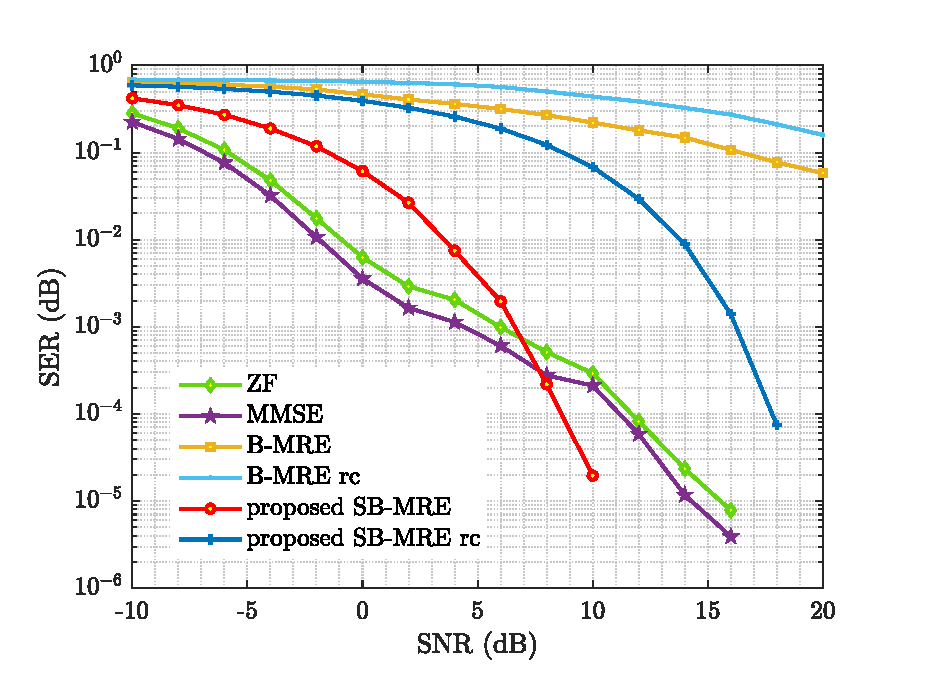
\includegraphics[width=.8\linewidth]{figures/performance.eps}
    \caption{So sánh $\operatorname{SER}$ của thuật toán đề xuất SB-MRE với các phương pháp nhận dạng tuyến tính.}
    \label{fig:performance}
\end{figure}

Tiếp đến, để kiểm chứng sự ảnh hưởng của số lượng ký hiệu pilot ($N_p$) đến hiệu suất của phương pháp đề xuất SB-MRE và SB-MRE rc, $\operatorname{SER}$ tương ứng với các $N_p$ được mô phỏng và đưa ra trong hình~\ref{fig:vary_N_p}. Số lượng pilot được thay đổi từ $N \rightarrow N_s/4$ tương ứng là $10\rightarrow 64$ và $\operatorname{SNR}$ được cố định là $5, 10$ hoặc $15$~dB. Dễ nhận thấy, khi số lượng ký hiệu pilot và $\operatorname{SNR}$ tăng thì $\operatorname{SER}$ sẽ giảm, tuy nhiên độ suy giảm là khác nhau. Với SB-MRE rc, tỷ lệ lỗi ký hiệu sẽ giảm nhanh khi $N_p$ tăng từ $10 \rightarrow 20$ ký hiệu, và giảm chậm và gần như hội tụ khi $N_p$ tiếp tục tăng lên đến 64. Các mức $\operatorname{SNR}$ lớn hơn sẽ cho $\operatorname{SER}$ tốt hơn và có thể đạt thấp hơn $10^{-2}$ cho SB-MRE giảm chi phí với $\operatorname{SNR}=15$~dB, $N_p > 20$ ký hiệu. Với SB-MRE, trước hết hiệu suất của SB-MRE sẽ vượt trội trên $10^1$~dB so với SB-MRE đã giảm chi phí ở tất cả các giá trị $\operatorname{SNR}$ khác nhau. Thứ hai, nhìn chung $\operatorname{SER}$ sẽ giảm dần đều ở tất cả các giá trị $N_p$. Thứ ba, độ dốc của các đường $\operatorname{SER}$ là tăng dần với $\operatorname{SNR}$ lớn hơn. Ở giá trị $\operatorname{SNR}=15$~dB, chỉ cần $31$ ký hiệu pilot để SB-MRE đạt được $\operatorname{SER}$ tuyệt đối. Tóm lại, số lượng pilot ảnh hưởng lớn đến độ chính xác của SB-MRE và ít hơn cho SB-MRE rc.
\begin{figure}[ht]
    \centering
    \begin{subfigure}
         \centering
         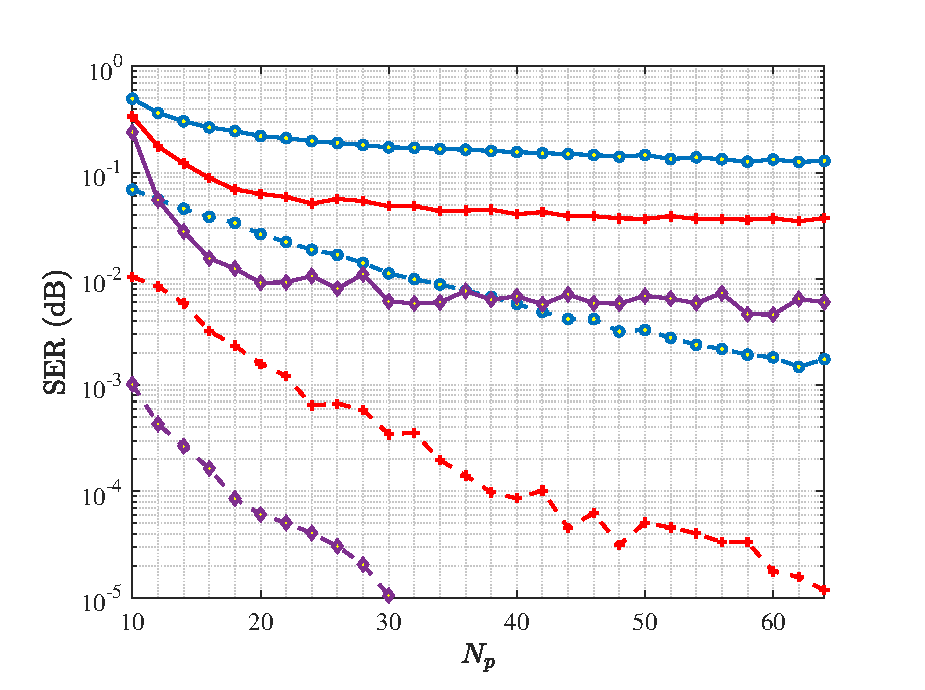
\includegraphics[width=0.8\linewidth]{figures/vary_N_p_1.eps}
     \end{subfigure}
     \hfill
     \begin{subfigure}
         \centering
         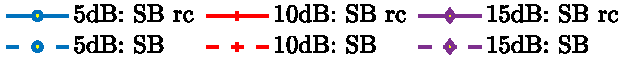
\includegraphics[width=.6\linewidth]{figures/legend.pdf}
     \end{subfigure}
     \hfill
    \caption{So sánh $\operatorname{SER}$ của thuật toán đề xuất SB-MRE với các số lượng pilot ($N_p$) và $\operatorname{SNR}$ khác nhau.}
    \label{fig:vary_N_p}
\end{figure}

Cuối cùng, ảnh hưởng của thành phần B-MRE trong SB-MRE sẽ được khảo sát thông qua trọng số $\lambda$. Trên hình~\ref{fig:vary_lambda}, hai phương pháp được đề xuất SB-MRE và SB-MRE rc sẽ được mô phỏng với các $\lambda$ và $\operatorname{SNR}$ khác nhau. Cụ thể, giá trị $\lambda$ sẽ được thay đổi trong khoảng $0,01 \rightarrow 0,2$ với bước $0,01$ và $\operatorname{SNR}$ được cố định là $5, 10$ hoặc $15$~dB. Có thể thấy rằng, $\operatorname{SER}$ của SB-MRE và SB-MRE rc không bị ảnh hưởng bởi $\lambda$ nhiều như số lượng pilot. Đặc biệt khi $\operatorname{SNR}$ thấp như $5$~dB, $\operatorname{SER}$ giảm rất ít khi $\lambda$ tăng, do ảnh hiệu suất của B-MRE ở các mức $\operatorname{SNR}$ thấp như đã khảo sát trên hình~\ref{fig:performance}. Khi $\operatorname{SNR}$ cao hơn như $10$~dB, B-MRE bắt đầu ảnh hưởng đến độ chính xác chung, đặc biệt là với SB-MRE khi ước lượng toàn bộ $K$ bộ làm bằng khi độ dốc của đường $\operatorname{SER}$ là rõ ràng hơn. Tuy nhiên, phải đến khi $\operatorname{SNR}=15$~dB, B-MRE mới thực sự gây ra ảnh hưởng, đường $\operatorname{SER}$ của SB-MRE rc giảm rõ rệt từ $10^{-3} \rightarrow 10^{-4}$ khi $\lambda$ tăng lên. Ở mức $\operatorname{SNR}$ này, SB-MRE đã đạt độ chính xác tuyệt đối chỉ với thành phần pilot $N_p = 32$ như đã khảo sát trên hình~\ref{fig:performance} và~\ref{fig:vary_N_p} nên không được biểu diễn trên hình~\ref{fig:vary_lambda}. Qua đó, có thể nhận xét trọng số của thành phần mù có ảnh hưởng đến độ chính xác của SB-MRE nhưng chỉ khi tỷ lệ tín hiệu tạp âm ở mức cao để thành phần mù bắt đầu cho thấy tác dụng.

\begin{figure}
    \centering
    \begin{subfigure}
         \centering
         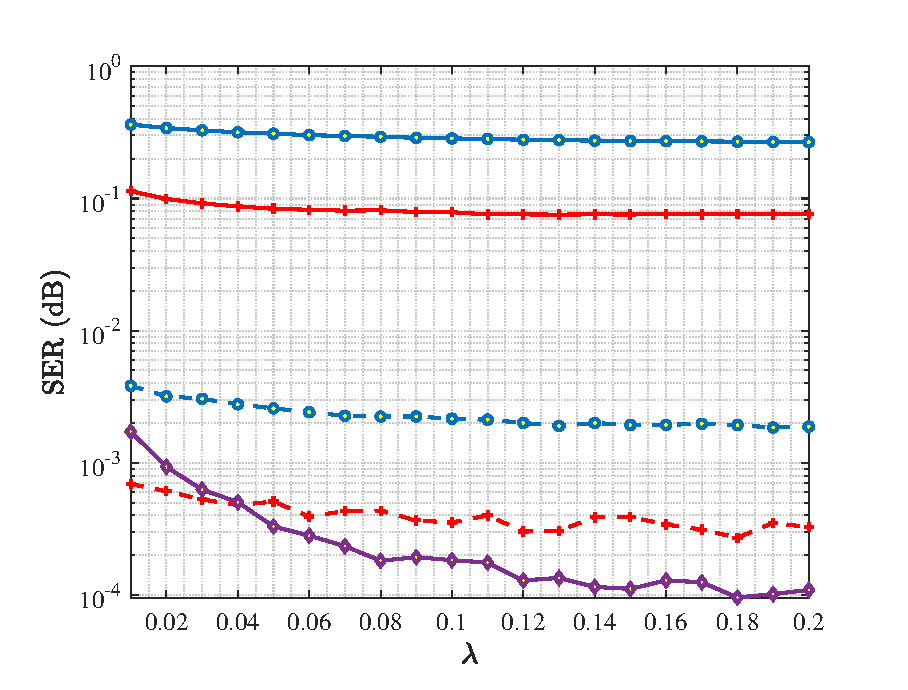
\includegraphics[width=.8\linewidth]{figures/vary_lambda.eps}
     \end{subfigure}
     \hfill
     \begin{subfigure}
         \centering
         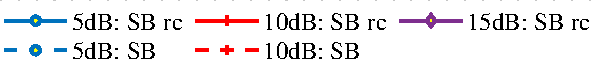
\includegraphics[width=.6\linewidth]{figures/legend_1.pdf}
     \end{subfigure}
     \hfill
    \caption{So sánh $\operatorname{SER}$ của thuật toán đề xuất SB-MRE với trọng số thành phần B-MRE ($\lambda$) và $\operatorname{SNR}$ khác nhau.}
    \label{fig:vary_lambda}
\end{figure}

\section{Kết luận chương}

Trong chương này, một kỹ thuật nhận dạng kênh truyền sử dụng thuật toán SB-MRE do chúng tôi đề xuất đã được trình bày. Trước hết, tác giả đã trình bày ngắn gọn lại phương pháp B-MRE truyền thống sử dụng cho các hệ thống truyền thông MIMO. Sau đó, phương pháp SB-MRE được đề xuất bằng các kết hợp thông tin từ một số ký hiệu pilot trong chuỗi ký hiệu và thông tin từ thành phần B-MRE kể trên. Các phương pháp giảm thiểu chi phí của thuật toán SB-MRE cũng được làm rõ, bao gồm, giảm thiểu độ phức tạp của thành phần B-MRE thông qua việc giảm số lượng bộ lọc cần ước lượng và giảm số lượng số ký hiệu pilot cần sử dụng. Các kết quả mô phỏng đã chỉ ra hiệu suất của phương pháp SB-MRE được đề xuất là khá vượt trội khi so sánh với các thuật toán nhận dạng hệ thống tuyến tính cổ điển và B-MRE gốc. Các mô phỏng cũng được thực hiện để xác nhận sự ảnh hưởng của số lượng ký hiệu pilot và đóng góp của thành phần mù đến độ chính xác của thuật toán SB-MRE ở các mức $\operatorname{SNR}$ khác nhau. Từ đó, có thể thấy phương pháp SB-MRE là tiềm năng cho các hệ thống truyền thông MIMO/mMIMO khi vừa giảm được số lượng ký hiệu pilot cần cho việc nhận dạng hệ thống mà vẫn giữ được một độ chính xác chấp nhận được.